\section{Meta Optimization Approach}
After the FMO step is developed and encapsulated, one may modify the weights used for the FMO iteratively until a condition is met or for a given number of steps.
We will, therefore, have one inner optimization (the FMO) and one outer optimization.
\begin{center}
	\begin{minipage}{.55\linewidth}
		\begin{algorithm}[H]
			\caption{Meta Optimization Algorithm Outline}
			\label{alg:meta_optim}
			\begin{algorithmic}
				\State initialize $w$
				\Repeat
					\State initialize $\mathbf{b}$ \Comment{FMO starts}
					\Repeat
						\State \textcolor{Prune}{ $\mathbf{d} = \textbf{L}\mathbf{b}$ \Comment{differentiable} }
						\State \textcolor{Prune}{ $c = C(w, \mathbf{d})$ \Comment{differentiable} }
						\State \textcolor{Prune}{ back-propagate $c$ }
						\State \textcolor{Prune}{ update $\mathbf{b}$ }
					\Until{\textit{FMO \textbf{stop condition}}} \Comment{FMO ends}
					\State update $w$
				\Until{\textit{Meta-optimization \textbf{stop condition}}}
			\end{algorithmic}
		\end{algorithm}
	\end{minipage}
\end{center}
% add algo illustration
The outer optimization step is not differentiable (or at least not in a reasonable computation time).
Hence, we will be looking at gradient-free optimization methods.

\subsection{Expert Weight Adjustment}
Expert systems are computer systems emulating the decision-making of a human expert.

\paragraph{Simple Weight Increase}
One approach involves increasing the weight of all unsatisfied constraints after each FMO optimization step.
This method is advantageous due to its simplicity in terms of implementation and understanding.
However, a significant limitation arises when none of the constraints are met, causing the outer optimization loop to stagnate.
In such cases, the optimization process remains stationary, usually when too many constraints are enforced.
This stationary state arises particularly in complex scenarios with multiple competing constraints and can result in a situation where progress is hindered, preventing the solution from improving over iterations.

\paragraph{Inverse Proportional Weight Increase}
Another approach involves increasing the weight of each constraint inversely proportional to how close it is to being met, thereby quantifying the degree of constraint satisfaction.
For instance, the degree of satisfaction can be quantified by calculating the area between the dose-volume histogram (DVH) constraint and the actual DVH curve; when this area is zero, the constraint is considered fully satisfied.
% add plot of the area between constraint lines and DVH curve
While this method remains relatively straightforward to implement and provides a more refined adjustment of weights based on how close each constraint is to being met, it can lead to oscillation issues.
Constraints may fluctuate between being satisfied and violated across iterations, hindering stable convergence.
Although adding momentum to the optimization process could mitigate these oscillations, expert systems of this nature typically require continuous tuning and refinement.
As a result, this approach may not be viable for reliable clinical applications where consistent performance is essential.

\subsection{Metric-Based}
Here, we suppose that one can construct a measure of the quality of a plan.

\paragraph{Hill Climbing}
Hill climbing \cite{skienna2008} is a simple optimization technique in which the solution iteratively moves toward an improved solution based on a defined metric.
In the context of radiotherapy treatment planning, several metrics have been proposed to quantify the quality of a plan, including Normal Tissue Complication Probabilities (NTCP), target coverage, conformity index, and heterogeneity index, among others \cite{lyman_normal_1992,li_input_2022} \label{metrics}.
This approach offers a systematic way to improve treatment plans by optimizing the chosen metric.

However, defining the correct metric of interest is challenging, as no single metric, nor a combination of metrics, has consistently proven to satisfy radio-oncologists' requirements.
In practice, the most reliable method for assessing the quality of a treatment plan remains the manual evaluation of dose-volume histograms (DVHs), which provide a detailed representation of the dose distribution across both the target and the surrounding organs at risk.

\paragraph{Pareto Exploration}
Researchers have developed algorithms to explore the Pareto surface of dose distributions, yet no consensus has been reached on selecting an optimal dose from this surface.
Consequently, Pareto surface exploration is unsuitable due to the absence of an objective quantitative measure for evaluating the quality of a specific plan \cite{huang_pareto_2021}.
This limitation similarly constrains other meta-optimization techniques, as they also rely on the availability of a clear, impartial criterion for plan evaluation \cite{wu_optimization_2001, xing_optimization_1999}.

\paragraph{Contextual Knowledge}
Another challenge is the varying difficulty across patients due to their different organ geometry.
In "easy" cases, clinicians may require a highly optimized dose distribution regarding the previously mentioned metrics.
On the other hand, for "harder" cases, they can afford to be more lenient regarding constraint satisfaction.

This context-aware acceptability criterion adds complexity to the optimization process.
It becomes challenging to define general rules not only for ranking treatment plans but also for deciding a plan's acceptability.



%%%%%%%%%%%%%%%%%%%%%%%%%%%%%%%%%%%%%%%%%%%%%%%%%%%%%%%%%%%%%%%%%%%%%%%%
%                                                                      %
%   %%%%%%%%%%%%%%%%%%%%%%%%%%%%%%%%%%%%%%%%%%%%%%%%%%%%%%%%%%%%%%%%   %
%   %%%%%%%%%%%%%%%%%%%%%%%%%%%%%%%%%%%%%%%%%%%%%%%%%%%%%%%%%%%%%%%%   %
%   %%%%%%%%%%%%%%%%%%%%%%%%%%%%%%%%%%%%%%%%%%%%%%%%%%%%%%%%%%%%%%%%   %
%   %%%%%%%%%%%%%%%%%%%%%%%%%%%%%%%%%%%%%%%%%%%%%%%%%%%%%%%%%%%%%%%%   %
%                                                                      %
%%%%%%%%%%%%%%%%%%%%%%%%%%%%%%%%%%%%%%%%%%%%%%%%%%%%%%%%%%%%%%%%%%%%%%%%



% Full paper:
% https://github.com/pauldubois98/AIME2024/blob/main/llncs_formatting.pdf
\section{Radiotherapy Dose Optimization via Clinical Knowledge Based Reinforcement Learning (AIME 2024)}

\subsection{Introduction}
Reinforcement learning (RL) is a machine learning paradigm that trains agents to make sequential decisions in dynamic environments \cite{brooks_what_2021}.
Agents learn to optimize their actions to achieve long-term objectives through trial and error guided by rewards or penalties.
The decisions taken by dosimetrists when optimizing treatment can be formalized as an RL problem.
Moreover, dosimetrists can guide the TPS towards an acceptable plan but usually can not explain their decision while interacting with the TPS.
The difficulty in explaining why certain decisions are taken suggests using deep RL over expert-based methods.
This setup is similar to image recognition, where one can say a picture represents a car or a boat but struggles to explain why.

The study’s primary hypothesis is that all the information needed to decide how to change the weights in the objective function relies on the Dose Volume Histograms (DVHs).
The fact that dosimetrists almost solely use DVH plots supports our hypothesis.
In order to learn the actions of dosimetrists who use a TPS to optimize doses, we leverage deep learning.
We train an agent that takes the DVHs as the input of the current optimized dose and predicts the evaluation of possible weight changes.

Access to the exact actions taken by human dosimetrists on the TPS is typically unavailable (as clinics do not usually store this data; only the final plan is held).
Therefore, we only use the dose distributions of previously treated patients to train our model.
This partial availability of data suggests the use of RL.

\paragraph{Reinforcement Learning Paradigm}
\begin{figure*}
	\centering
	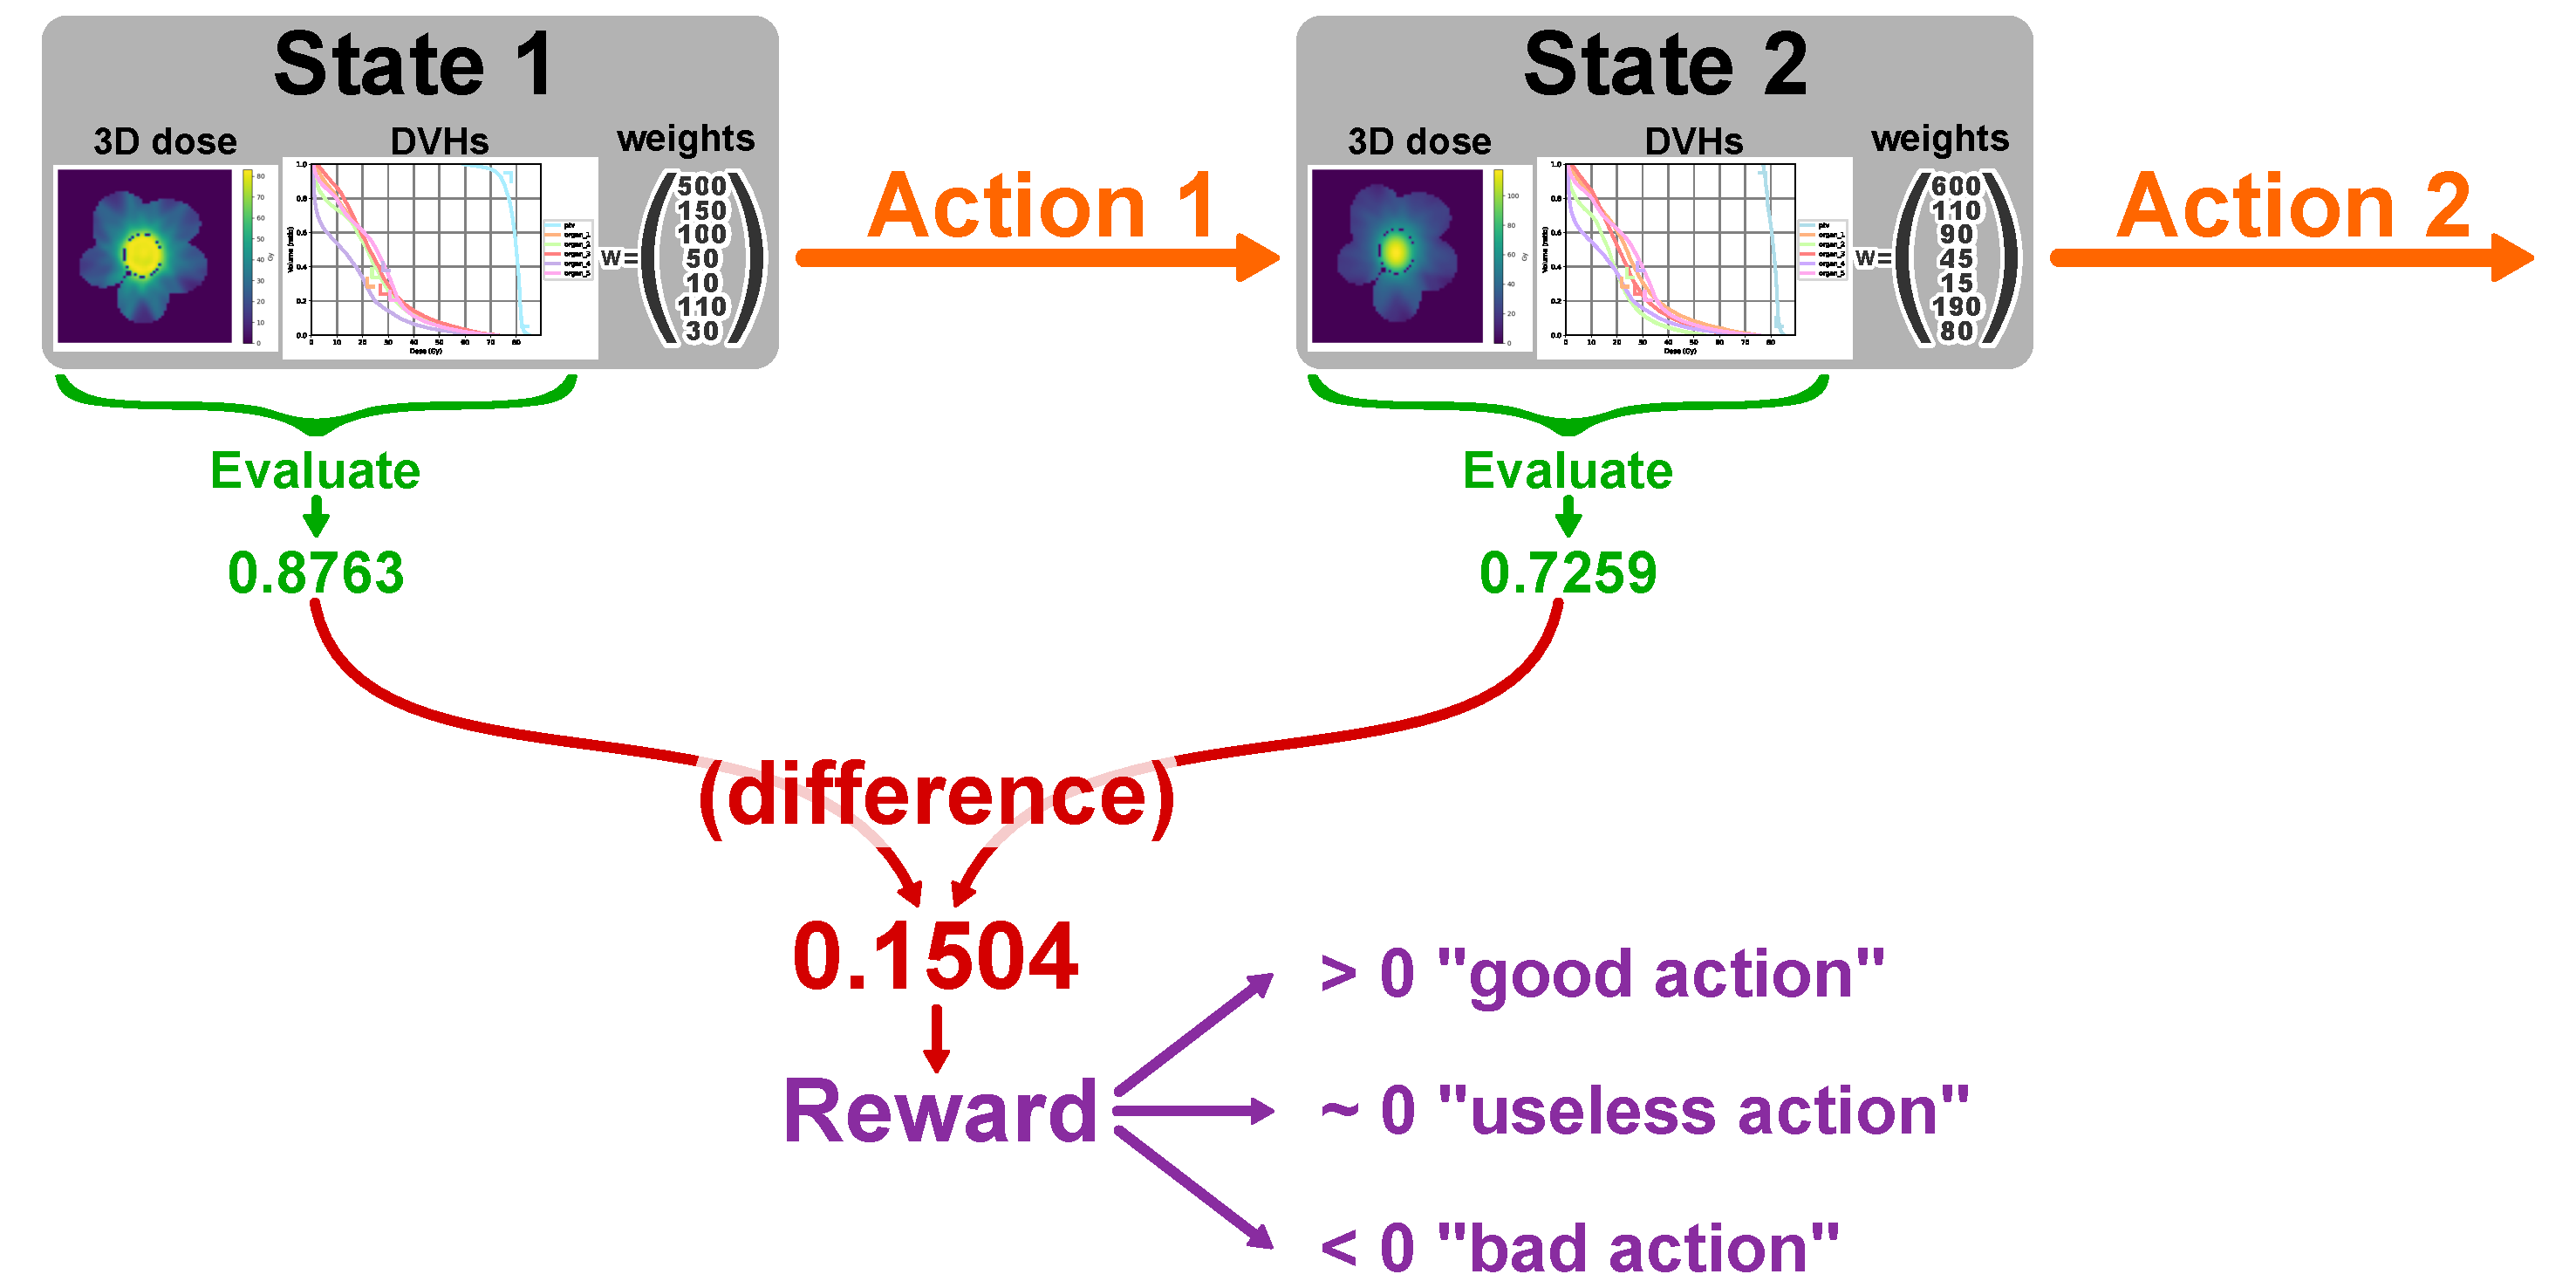
\includegraphics[width=0.9\textwidth]{AIME/reward.pdf}
	\caption{Classical reinforcement learning reward for automatic dosimetry.}
	\label{fig:reward_fig}
\end{figure*}

In classical RL, we want $V(S_t) = R_t + \gamma V(S_{t+1})$.
(so the update is $V(S_t) \leftarrow (1-\alpha) V(S_t) + \alpha \left[ R_{t+1} + \gamma V(S_{t+1}) \right]$).
In the context of dose optimization, the reward $R_t$ is defined as $R_t = \mathcal{E}(S_{t+1}) - \mathcal{E}(S_t)$, where $\mathcal{E}$ is a function that evaluates the quality of a state (such that higher is better; if lower is better, then swap $s_t$ and $S_{t+1}$).

The evaluation $\mathcal{E}$ can be one or a mixture of the metrics mentioned in the introduction (Section \ref{metrics}) \cite{shen_hierarchical_2021} \cite{shen_intelligent_2019} \cite{moreau_reinforcement_2021}.
This setup may leverage knowledge about which actions to perform instead of guessing randomly, as a meta-optimizer would do.
Hence, the RL could gain some computation time compared to a meta-optimization.

However, this technique does not use past plans; it only needs the optimizer inputs (CT, structures contours).
We propose using the availability of past treatment plans to more accurately reflect the complexity of decisions made by dosimetrists and better match their expectations of a fully automatic treatment planning system.

\subsection{Methods}
We present a novel paradigm for reward-based RL agents in dosimetry.
This revised reward framework better reproduces human-optimized dose distributions.

\paragraph{Reinforcement Learning Reward}
As developed in previous work, we can derive a distance between dose plans \cite{paul_dubois_novel_2024}.
If we consider the clinical dose of past cases (used for training) as the best achievable one, we can evaluate a dose plan by computing its distance from the clinical dose plan.

Let $D_t$ be the dose associated with $S_t$, and $D_C$ the clinical dose.
We then define $\mathcal{E}(S_t) = \mathcal{D}(D_t, D_C)$.
Since, in that case, $\mathcal{E}(S_t)$ should be minimized, we will define the reward as $$R_t = \mathcal{E}(S_t) - \mathcal{E}(S_{t+1}) = \mathcal{D}(D_t, D_C) - \mathcal{D}(D_{t+1}, D_C).$$
This reward can be interpreted as the "distance gained to the clinical dose". 

\paragraph{Architecture}
We use a dense neural network, which inputs the DVHs and current normalized weight values.
It outputs the $Q(s, a)$ value for each possible action $a$.
Dense layers are very prone to overfitting.
In order to force the network to actually predict the following evaluation for each possible action, without overfitting, we incorporated a bottleneck in the network (Figure \ref{fig:architecture}).
Compressing the information stops the network from overfitting.
Networks with such architecture show very little difference between training and validation sets (see Figure \ref{fig:losses_training}).

\begin{figure*}
	\centering
	\begin{subfigure}{0.48\linewidth}
		\centering
		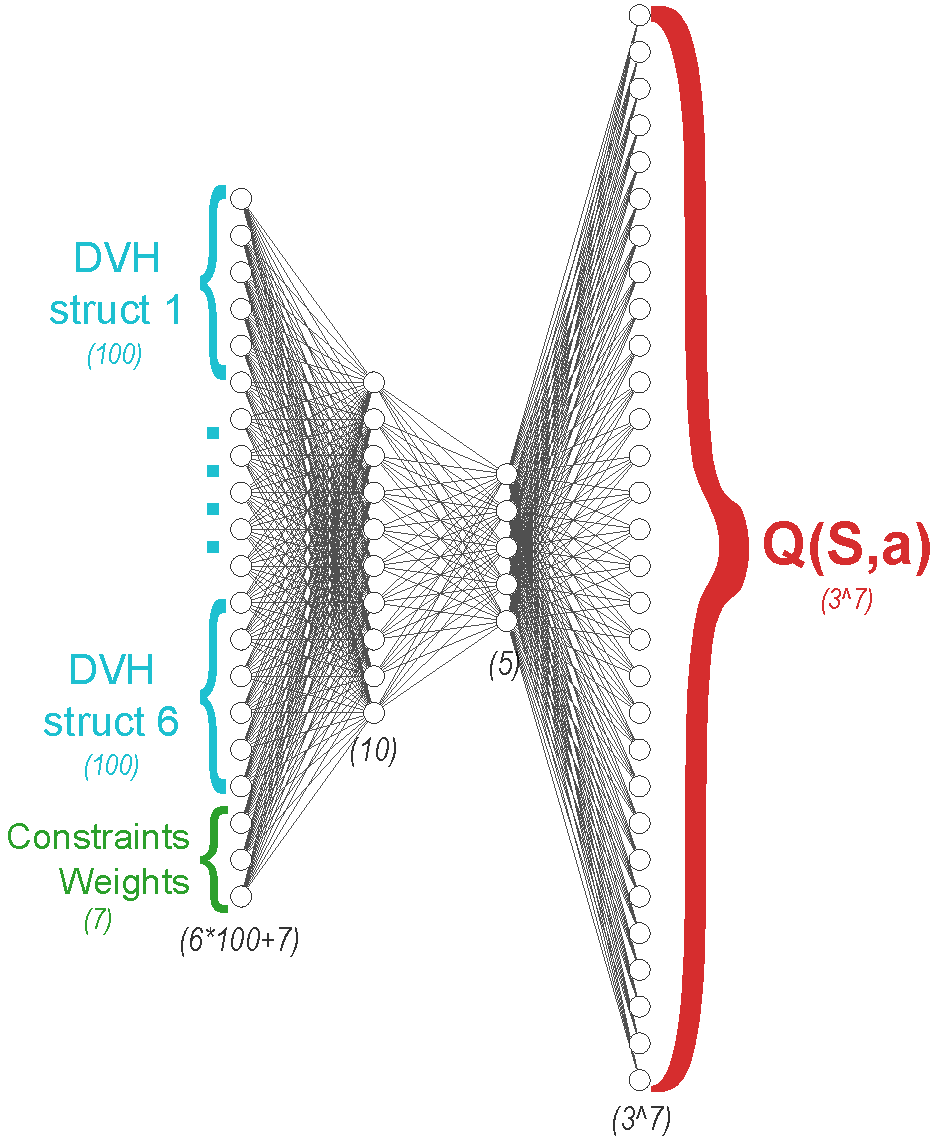
\includegraphics[height=8cm]{AIME/architecture_all_actions.pdf}
		\caption{Architecture.}
		\label{fig:architecture}
	\end{subfigure}
	\begin{subfigure}{0.48\linewidth}
		\centering
		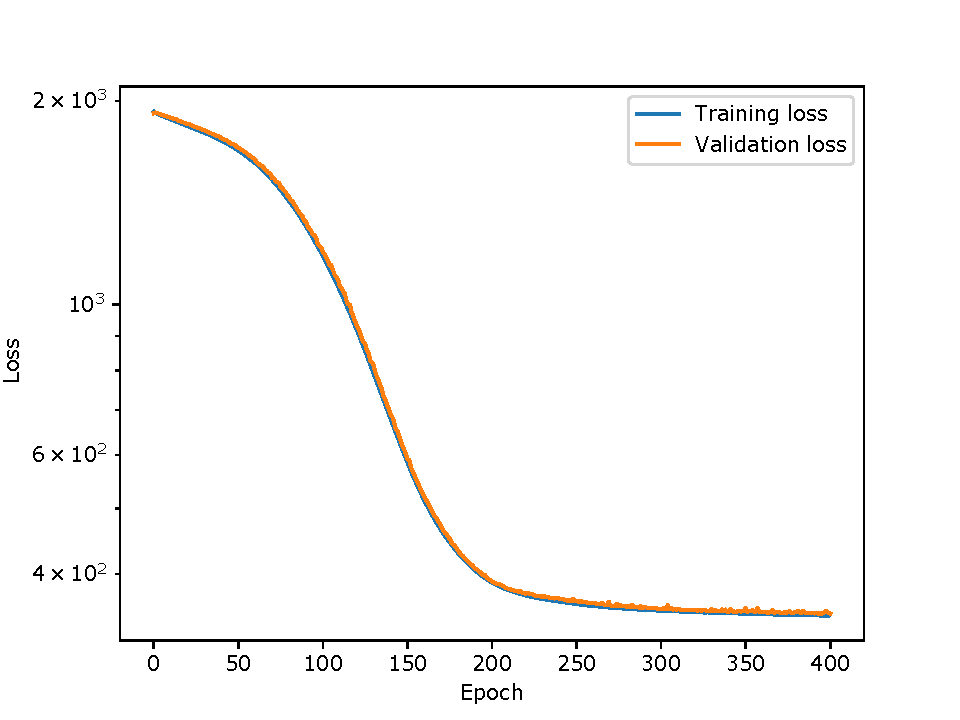
\includegraphics[height=7cm]{AIME/losses-distance.pdf}
		\caption{Loss during training.}
		\label{fig:losses_training}
	\end{subfigure}
	\caption{Deep neural network used for the RL agent.}
\end{figure*}

\paragraph{Avoiding Off-Distribution}
We generated a training set of over 125k actions (this took five days on an NVIDIA GeForce GTX 1080).
Despite this relatively large dataset, we have not explored exhaustively the state-actions space, and the network still lands off-distribution.
This can easily be spotted when the predicted $Q$ value is greater than the current distance to the clinical dose; we choose to ignore those predictions, and in fact all outlier predictions.
The justification is that our set of actions is limited, no action will suddenly drastically improve the plan.
It is the combination of several sequential actions that allows good plan optimization.
Therefore, while testing, we choose the action with the best prediction, while passing the outlier test just mentioned.

\paragraph{Data}
We generated synthetic phantom patients and corresponding clinically relevant dose distributions.
Variability can arise in clinical practice due to differences in organ contouring methods (manual or automated) and the potential for clinics to delineate different organs.
To mitigate this variability in our ongoing research, we employed synthetic patients, ensuring a standardized approach where all patients possess the same number of organs with similar shapes and identical prescription parameters.
Future studies will explore the application of this methodology to actual clinical cases.

\subparagraph{Synthetic patients}
We generated a cohort of 130 patients with bodies modeled as oval axial cross-sections, assigning a uniform density equivalent to water.
Within each body, we placed an ellipsoidal planning target volume (PTV) with a slightly different density, sampled from $\mathcal{N}(1,0.05)$.
Five organs at risk (OARs) were also positioned around the PTV, aligned along the axial plane.
The exact position and size of organs and PTV were randomized to consider the geometric variability across individuals.
This setup was designed to simulate cases analogous to typical prostate cancer scenarios.

\begin{figure}
	\centering
	\begin{subfigure}{0.48\linewidth}
		\centering
%		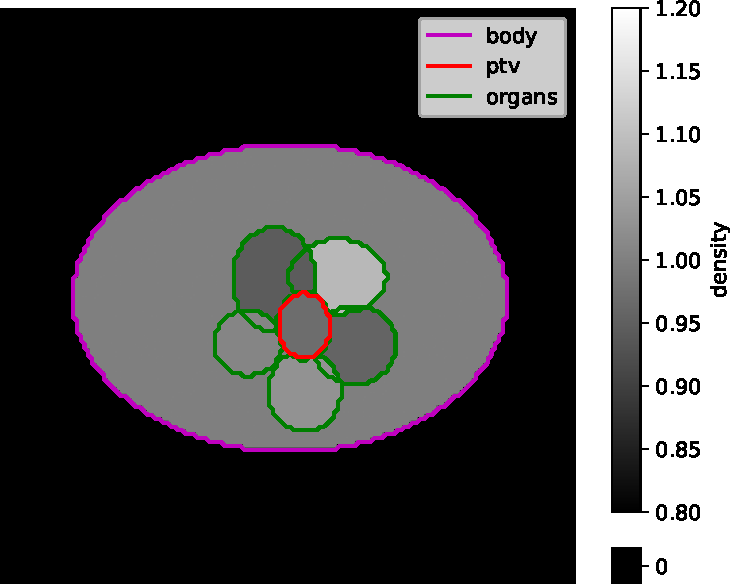
\includegraphics[height=5cm]{AIME/main_slice-ct.pdf}
		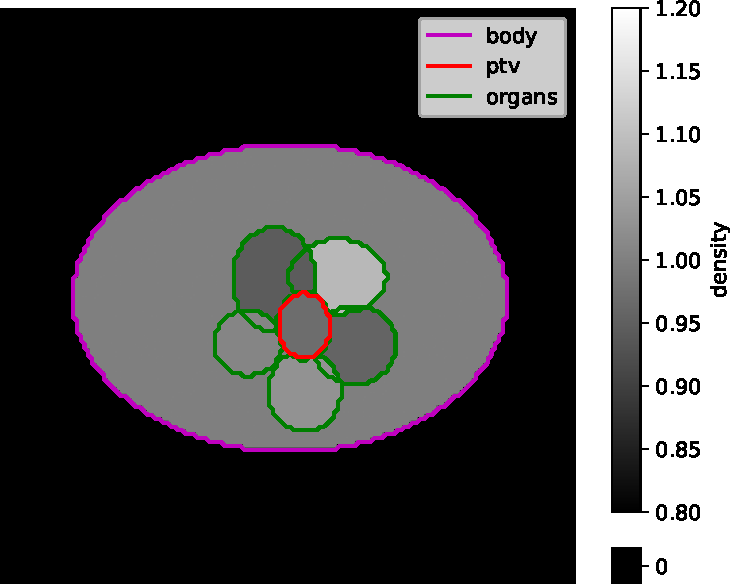
\includegraphics[width=\linewidth]{AIME/main_slice-ct.pdf}
		\label{fig:main_slice-ct}
		\caption{CT}
	\end{subfigure}
	\hfill
	\begin{subfigure}{0.48\linewidth}
		\centering
%		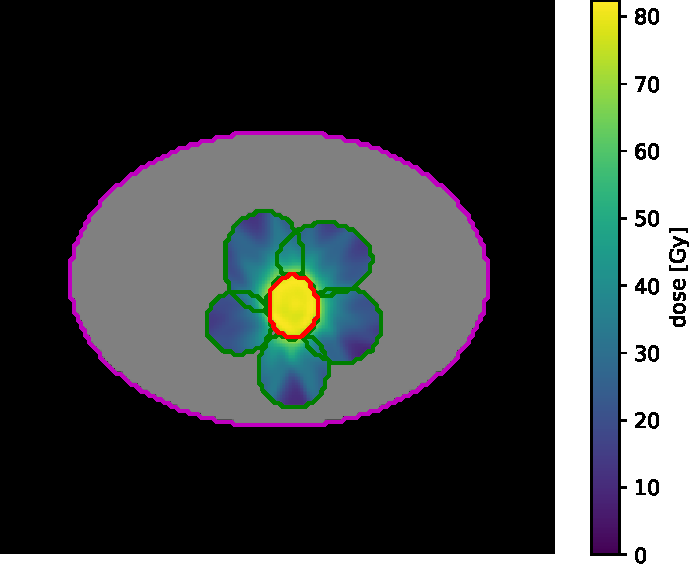
\includegraphics[height=5cm]{AIME/main_slice-dose.pdf}
		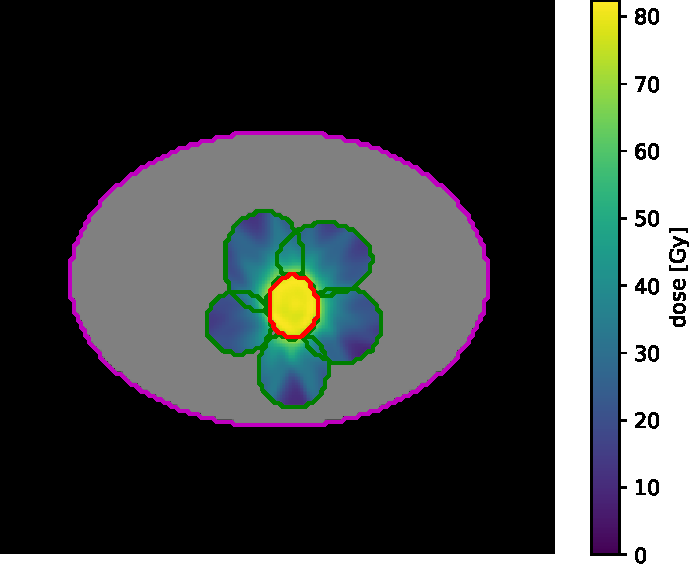
\includegraphics[width=\linewidth]{AIME/main_slice-dose.pdf}
		\label{fig:main_slice-dose}
		\caption{Clinical dose}
	\end{subfigure}
	\begin{subfigure}{\linewidth}
		\centering
		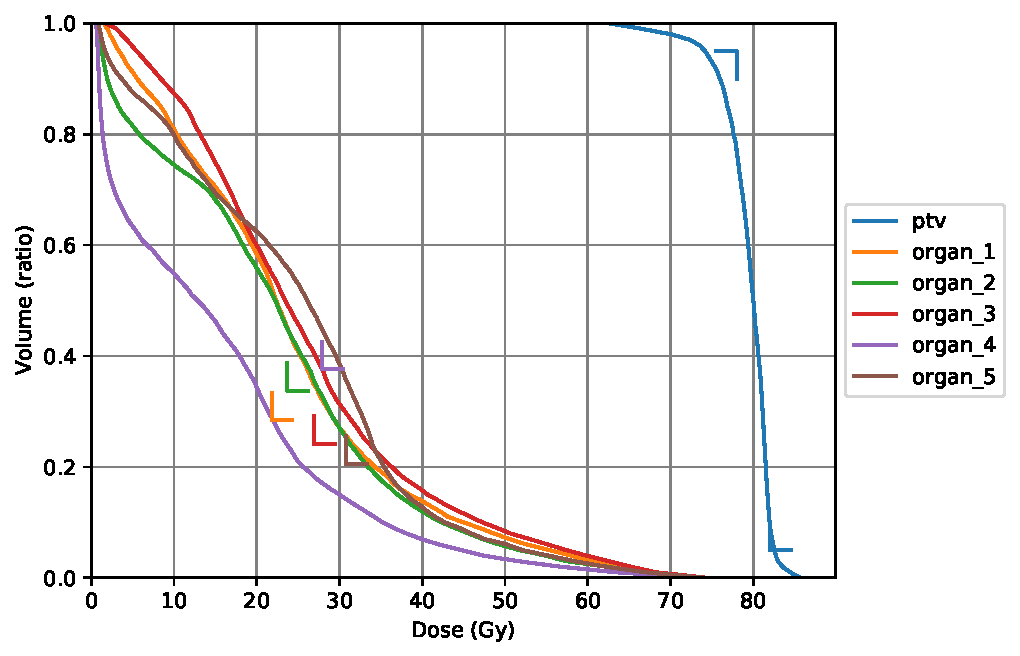
\includegraphics[width=0.8\linewidth]{AIME/dvh_example.pdf}
		\caption{Associated clinical dose \textbf{DVH}}
		\label{fig:clinical_dvh}
	\end{subfigure}
	\caption{Example of a (generated) patient's main axial slice (center of the PTV) and DVHs.}
\end{figure}

\subparagraph{Synthetic clinical dose}
After generating the patient's CT and structures, we needed to create a reference dose that our agent should mimic.
We manually set weights and performed a standard optimization.
The dose prescription is a standard $80\,\textit{Gy}$ on PTV, the same across all patients.
The table of the clinical DVH constraints used for optimization are detailed in table \ref{table:DVH_constraints}
We used a seven-beam IMRT irradiation technique on all the cohorts.

\begin{table}
	\begin{center}
		\begin{tabular}{| c | c | c | c |} 
			\hline
			Constraint type & Structure & Volume & Dose \\ 
			\hline
			Minimum & PTV & $95\,\%$ & $78.0\,\textit{Gy}$ \\
			Maximum & PTV & $5\,\%$ & $82.0\,\textit{Gy}$ \\
			Maximum & Organ 1 & $28.4\,\%$ & $21.8\,\textit{Gy}$ \\
			Maximum & Organ 2 & $33.7\,\%$ & $23.7\,\textit{Gy}$ \\
			Maximum & Organ 3 & $24.1\,\%$ & $26.9\,\textit{Gy}$ \\
			Maximum & Organ 4 & $37.6\,\%$ & $27.9\,\textit{Gy}$ \\
			Maximum & Organ 5 & $20.5\,\%$ & $30.8\,\textit{Gy}$ \\
			\hline
		\end{tabular}
	\end{center}
	\caption{
		DVH constraints used to create the cost function used in the FMO.
	}
	\label{table:DVH_constraints}
\end{table}

\subsection{Results}
Figure \ref{fig:distance} shows how the distance between our RL agents performs over five steps on 30 test patients (unseen during the training).
A lower distance is interpreted as an improved dose, since it is closer to the best dose, which is the clinical one.
\begin{figure*}
	\centering
	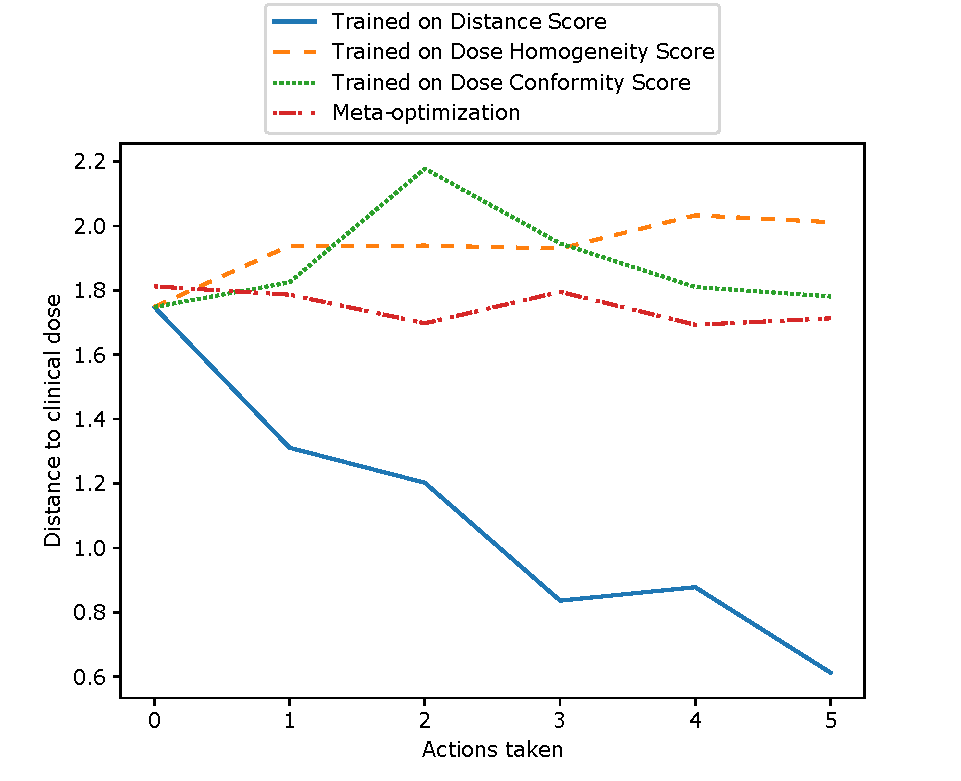
\includegraphics[width=0.7\textwidth]{AIME/DistanceToClinicalDose.pdf}
	\caption{Average distance between RL agent's dose and clinical dose.}
	\label{fig:distance}
\end{figure*}

\paragraph{Quantitative Results}
The network converged on the training data, and validation showed minor overfitting.
For testing, we generated 30 brand new cases that we again manually optimized.
We then used the RL model to perform the optimization of these 30 unseen cases.
On average, our model was able to reduce the dose distance with manually optimized dose by a factor of $~3$ (from $~1.8$ at iteration $0$ to $~0.6$ at iteration $4$), as shown in Table \ref{table:results}.

We remark from the Table \ref{table:results} that the homogeneity score and conformity score give similar results.
Classical meta-optimization performs well, but needs a metric to elect the best dose (during the test, the clinical dose is unknown, so the DVHs distance metric is not available).
We also observe that clinical doses are not always scoring high (in this test set, a high conformity, but low homogeneity compared to automatic techniques).
This show the difficulty to create a metric that capture all the complexity of a clinically acceptable dose.

\begin{table}
	\begin{center}
		\begin{tabular}{| c || c | c | c |} 
			\hline
			Agent $\backslash$ Metric & Mean Final Distance$^*$ & Homogeneity Score$^\dagger$ & Conformity Score$^\dagger$ \\ 
			\hline
			RL Distance Score & \textbf{0.612} & 1.871 & 0.406 \\ 
			RL Homogeneity Score & 2.012 & \textbf{4.387} & 0.567 \\
			RL Conformity Score &  1.770  & 4.017 & 0.507 \\
			Meta-optimization & N/A & 4.117 & \textbf{0.610} \\
			\textit{Clinical doses} & \textit{0} & \textit{1.541} & \textit{0.580} \\	
			\hline
		\end{tabular}
		\\
		$^*$ distance is imporved performance through a lower score.\\
		$^\dagger$ score is imporved performance through a higher score.
	\end{center}
	\caption{
		Average performances of four algorithms tested on DVHs distance to clinical dose, dose homogeneity-based score, and conformity-based score.
	}
	\label{table:results}
\end{table}

\paragraph{Qualitative Results}
Figure \ref{fig:steps} shows the DVHs at each of the first four optimization steps on one of the test patients, unseen by the agent during the training.
Our model drastically reduced the dose distance with manually optimized doses.
Visual inspection of the DVHs plot shows that the dose optimized by the RL agent is very close to the clinical (manually fine-tuned) one.

\begin{figure}
	\centering
	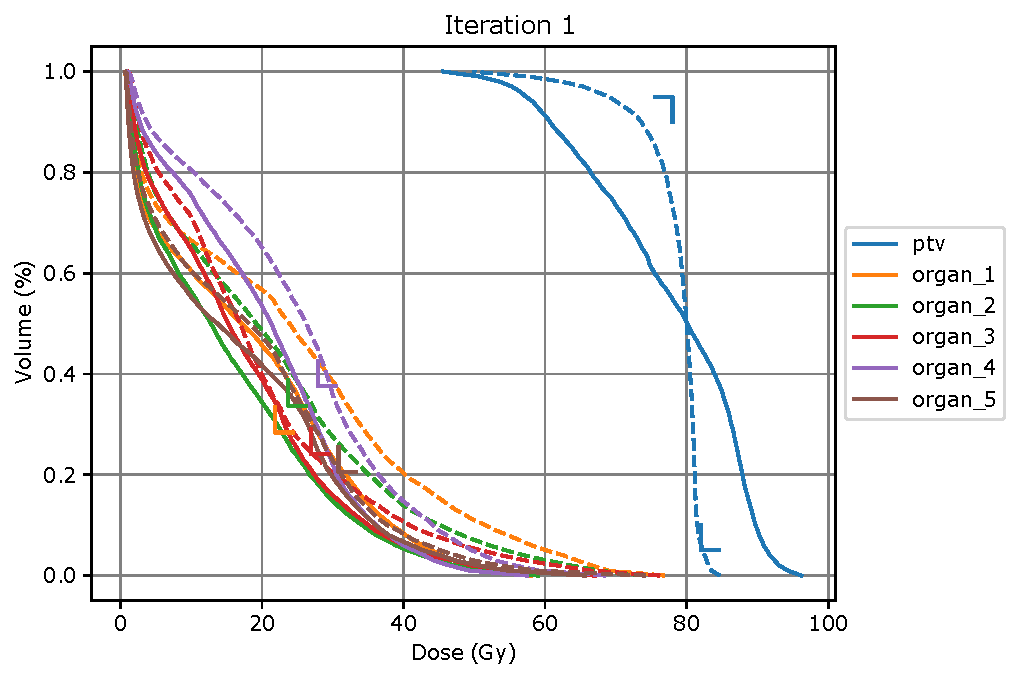
\includegraphics[width=0.49\textwidth]{AIME/distance-test-w1.pdf}
	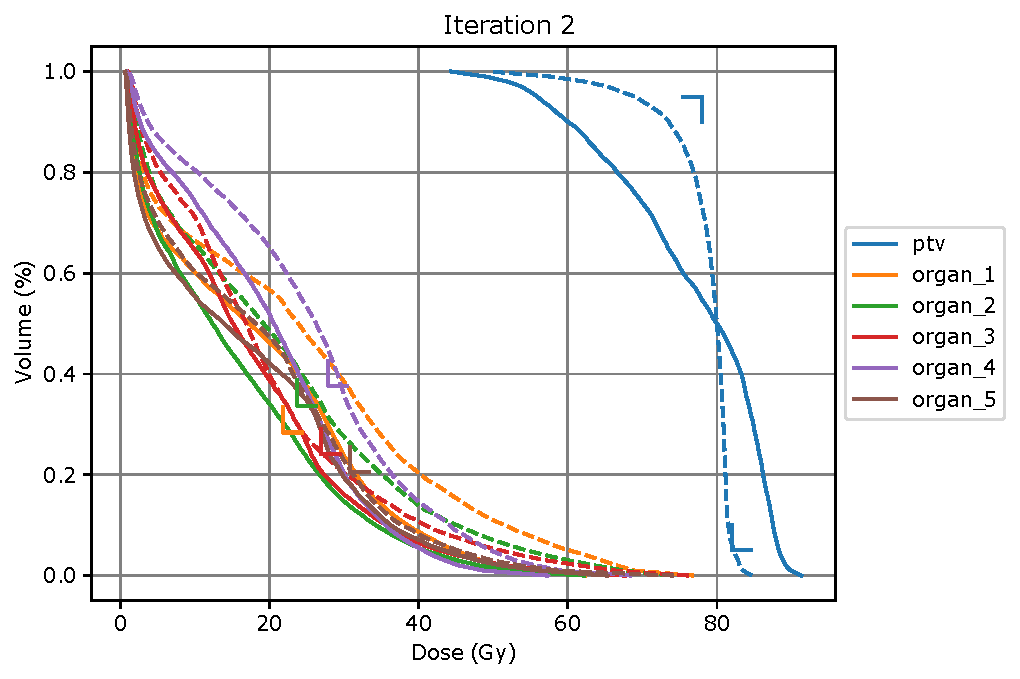
\includegraphics[width=0.49\textwidth]{AIME/distance-test-w2.pdf}
	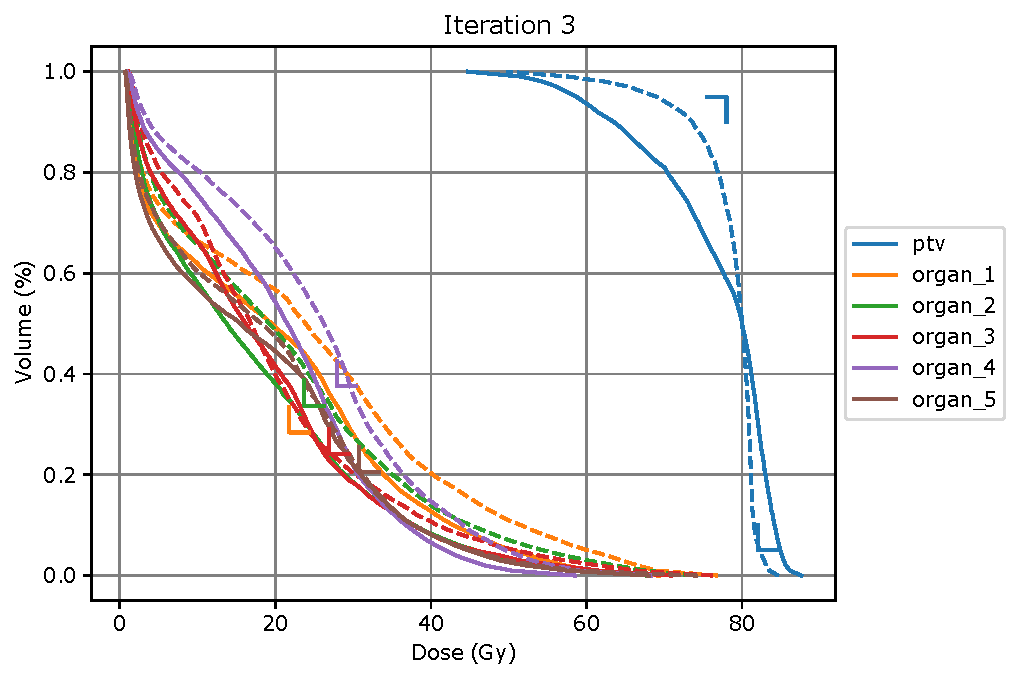
\includegraphics[width=0.49\textwidth]{AIME/distance-test-w3.pdf}
	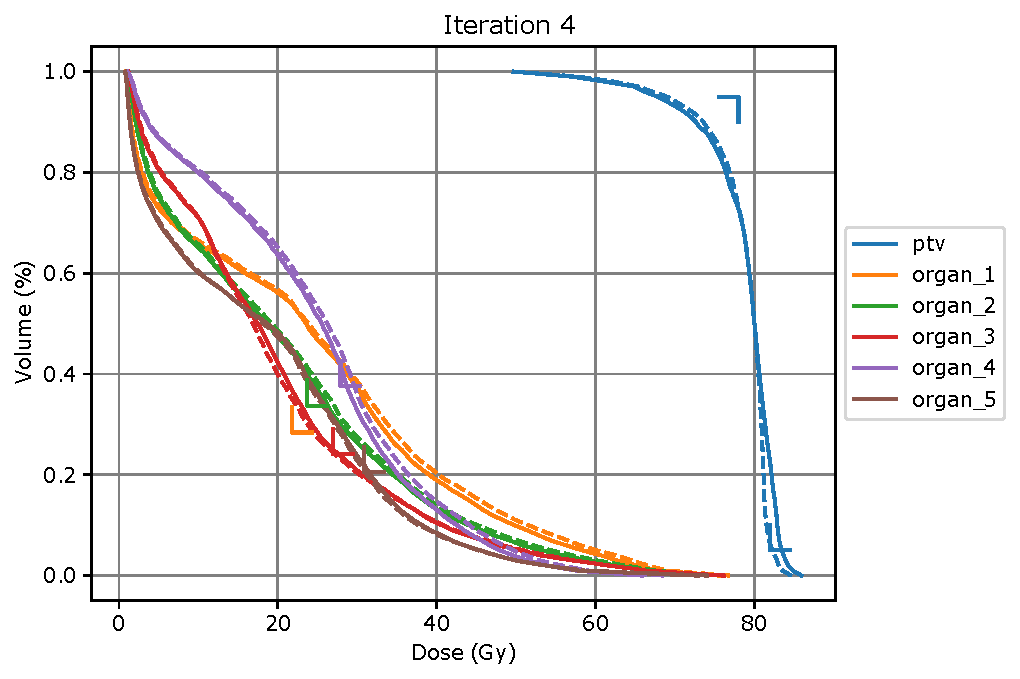
\includegraphics[width=0.49\textwidth]{AIME/distance-test-w4.pdf}
	\caption{
		RL Agent DVHs after each action taken on a test (unseen) patient.
		Solid lines are the agent's dose DVHs; dotted ones are the reference dose DVHs (manually fine-tuned).
	}
	\label{fig:steps}
\end{figure}

\subsection{Discussion and Conclusion}
Our study demonstrates the potential of deep RL for automating radiotherapy treatment plan optimization.
A key strength of our approach is its ability to learn from past treatment plans, capturing the complex decision-making processes of human dosimetrists.
This data-driven approach avoids the limitations of pre-defined metrics, which may not fully capture the nuances of optimal treatment planning.

However, our study also has limitations.
The agent's performance relies on the quality and quantity of available training data.
Cases with limited historical data or complex anatomical features may require additional strategies.
Moreover, while the agent achieves promising results regarding dose distance reduction, the dose is not guaranteed to be clinically acceptable.
Although this study demonstrates the promise of our RL approach in a controlled setting, one final limitation to mention is that extending it to real-world radiotherapy planning would necessitates addressing additional complexities and constraints.

Several avenues exist for further research.
Firstly, we plan to investigate strategies for incorporating additional information, such as patient characteristics and anatomical complexities, into the training process.
For example, a potential improvement to the current model involves the integration of 3D dose distributions as input.
This additional information would allow the RL agent to identify dose hotspots within the treatment volume better.
This spatial representation of dose delivery would enable the agent to more accurately assess areas of over- or under-dosage, leading to more informed decision-making during plan optimization.
Ultimately, the agent is expected to improve the clinical acceptability of the generated treatment plans by using a more comprehensive understanding of the dose landscape and its implications for treatment outcomes.

Secondly, we aim to explore techniques for improving the interpretability of the RL agent’s decision-making process.
Interpretability is essential for building trust in the system and facilitating its clinical adoption.
By developing techniques that allow dosimetrists and clinicians to understand the rationale behind the agent’s actions, we can ensure that its decisions align with clinical expertise and best practices.
This transparency will support the validation of the agent’s performance and provide insights into potential areas for refinement and further optimization.

Our approach differs from previous RL-based methods for radiotherapy planning in two key aspects.
First, we avoid relying on pre-defined metrics for evaluation, which can be subjective, and limit the agent's ability to learn complex optimization strategies.
Second, compared to traditional meta-optimization approaches, our method leverages past treatment data, potentially leading to more informed decision-making during the optimization process.

This study demonstrates deep RL's feasibility and potential benefits for automating radiotherapy treatment plan optimization.
Our approach is capable of directly predicts state evaluations, and shows promise in achieving significant improvements in efficiency and, potentially, treatment outcomes.
Further research is needed to address limitations, improve interpretability, and ensure safe clinical integration.
This approach could revolutionize radiotherapy planning, leading to more standardized, efficient, and improved patient care.



%%%%%%%%%%%%%%%%%%%%%%%%%%%%%%%%%%%%%%%%%%%%%%%%%%%%%%%%%%%%%%%%%%%%%%%%
%                                                                      %
%   %%%%%%%%%%%%%%%%%%%%%%%%%%%%%%%%%%%%%%%%%%%%%%%%%%%%%%%%%%%%%%%%   %
%   %%%%%%%%%%%%%%%%%%%%%%%%%%%%%%%%%%%%%%%%%%%%%%%%%%%%%%%%%%%%%%%%   %
%   %%%%%%%%%%%%%%%%%%%%%%%%%%%%%%%%%%%%%%%%%%%%%%%%%%%%%%%%%%%%%%%%   %
%   %%%%%%%%%%%%%%%%%%%%%%%%%%%%%%%%%%%%%%%%%%%%%%%%%%%%%%%%%%%%%%%%   %
%                                                                      %
%%%%%%%%%%%%%%%%%%%%%%%%%%%%%%%%%%%%%%%%%%%%%%%%%%%%%%%%%%%%%%%%%%%%%%%%



% Full abstract:
% https://github.com/pauldubois98/ASTRO2024/blob/main/abstract.pdf
\section{Clinically Dependent Fully Automatic Treatment Planning System (ASTRO 2024)}
In the previous section, we propose a novel approach using RL agents trained to mimic human optimization based on historical dose distributions from past treatments.
This section will show that the RL agent developed above method allows for clinic-specific optimization.
The RL agent adapts to various clinical practices without requiring additional information beyond the clinic's historical dose data.

% move to ccl?
% By tailoring the RL agent's training to the specific dose patterns previously delivered by a clinic, the agent can learn to replicate the clinic's internal standards and guidelines, making it possible to deploy the same training algorithm across multiple institutions.
% The system adapts automatically to each clinic's specific practices, thus overcoming the challenge of clinical variability and paving the way for broader adoption of fully automatic TPS in routine clinical settings.
% Our approach is tailored to each clinic’s specific treatment guidelines by training RL agents on historical treatment data from that clinic.
% The system is designed to mimic human dosimetrists' optimization strategies, thus providing plans that are aligned with the clinical practices of individual institutions.

\subsection{Purpose / Objective}
One area that remains challenging is the complete automation of treatment planning.
Current TPS technologies offer either manual treatment planning or a single automatic planning.
They fail to consider the wide variation in practices across clinics, which often leads to sub-optimal treatment plans according to one clinic-specific guideline.
Manual planning by dosimetrists remains how most treatment plans are calculated.

There is significant interest in developing a fully automatic TPS that can mimic human decision-making processes while remaining adaptable to different clinics' specific practices.
Reinforcement learning (RL) has emerged as a promising approach in automated planning because of its ability to adapt to complex environments and learn from interactions with them.
In radiotherapy, RL can theoretically adjust the weight of constraints in optimization to achieve clinically acceptable plans.
However, current RL systems have struggled to replicate the clinical guideline adaptability of human dosimetrists.

In this section, we propose a solution that leverages the clinic's past treatment data to train RL agents that can optimize treatment plans according to local clinical guidelines.
By training one agent per clinic, the system ensures that the RL agents adhere to each clinic's specific standards, potentially making automated TPS more clinically viable.
We hypothesize that our clinic-specific RL agents can optimize radiotherapy plans while adhering to the respective institutional standards.

\subsection{Materials/Methods}

\paragraph{Training Data}
We created three clinical doses for each patient, each following a specific guideline.
In order to reduce computation time (as this time, we had three different clinics for each patient), we generated a cohort of 50 virtual patients for training and another 20 for testing.
Each case was manually optimized to serve as a reference for the RL agent.

\paragraph{Reinforcement Learning Framework}
We use the same RL framework described in section \ref{reinforcement_learning_framework}, where the reward function was designed to penalize deviations from the reference dose distribution by comparing the RL-generated DVHs with those of the training cases.
The closer the agent’s plan was to the reference, the higher the reward received.
This approach differs from traditional RL reward systems that often struggle to provide meaningful feedback in complex medical scenarios like dosimetry, where the “goodness” of a plan is difficult to quantify with a single metric.
Most importantly, this approach allows the optimization to fit each center’s internal standard practices and guidelines.
We created three RL agents, each mimicking the treatment plans of a specific clinic.

\subsection{Results}

\paragraph{Qualitative Evaluation}
Figure \ref{fig:RL_clinics} summarizes the evolution of the average distance between the reinforcement learning agent’s dose and the dose from clinics A, B, and C throughout iterations of importance wights changes.
Each one of the three agents was trained on the dose data of one specific clinic.
Throughout iterations, RL agent were able to gradually reduce the distance with the dose they were trained to replicate.

\begin{figure}
	\centering
	\begin{subfigure}{0.32\linewidth}
		\centering
		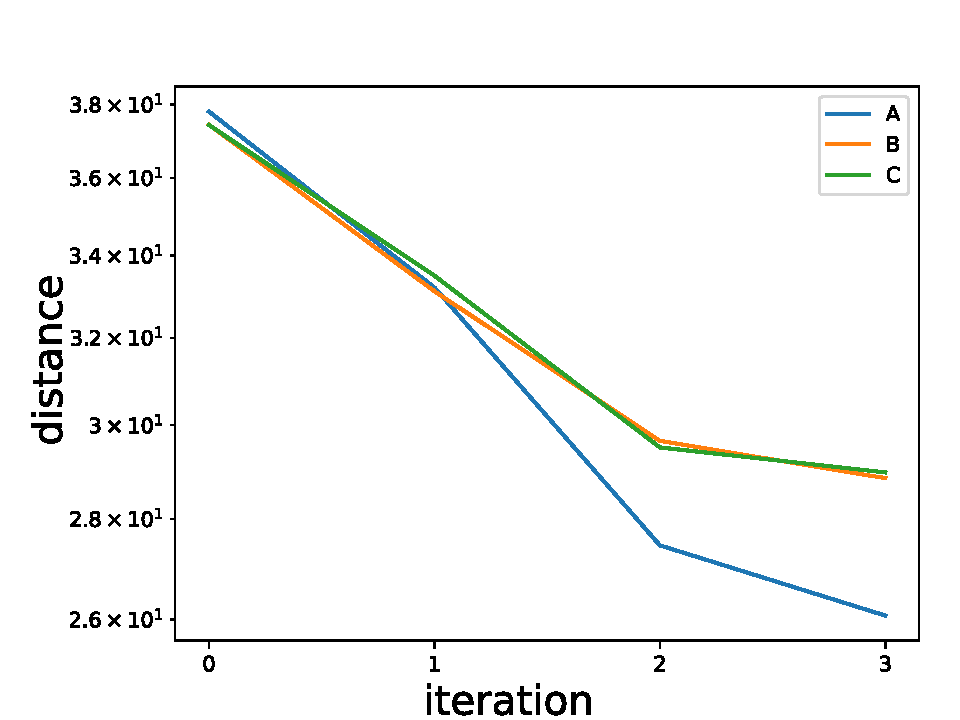
\includegraphics[width=\linewidth]{ASTRO/distanceA_semilogy.pdf}
		\caption{RL agent trained to replicate doses from clinic A.}
		\label{fig:RL_clinic_A}
	\end{subfigure}
	\hfill
	\begin{subfigure}{0.32\linewidth}
		\centering
		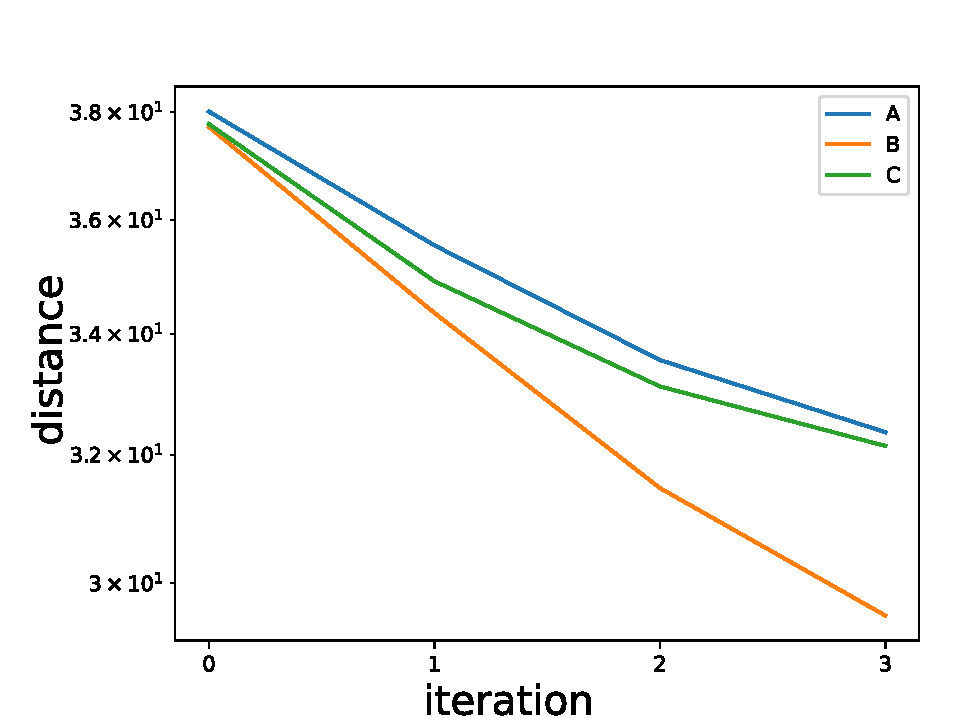
\includegraphics[width=\linewidth]{ASTRO/distanceB_semilogy.pdf}
		\caption{RL agent trained to replicate doses from clinic B.}
		\label{fig:RL_clinic_B}
	\end{subfigure}
	\hfill
	\begin{subfigure}{0.32\linewidth}
		\centering
		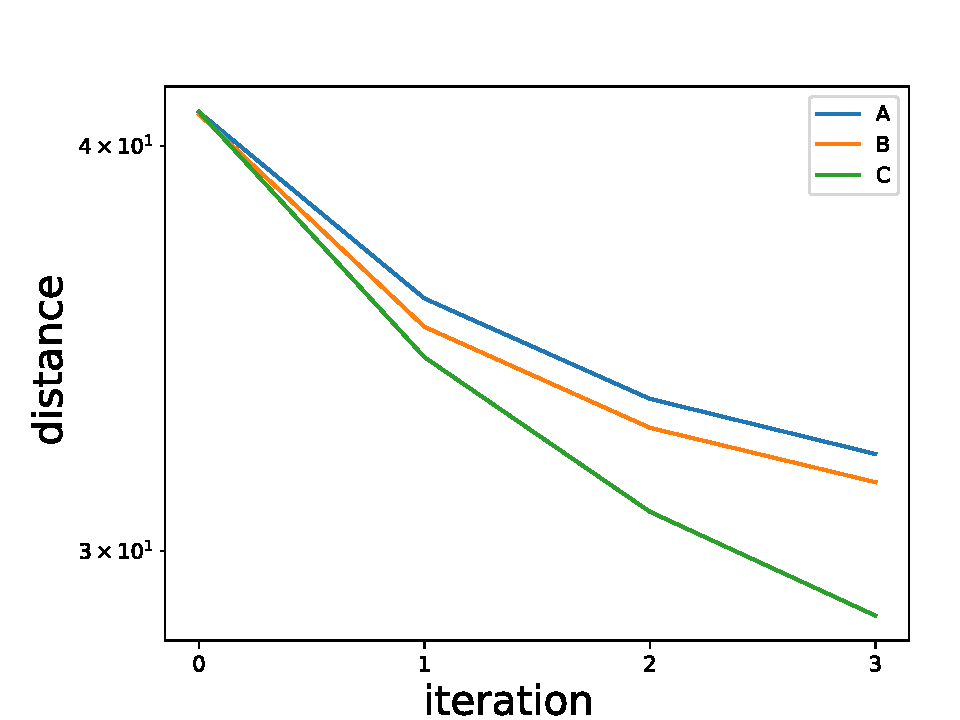
\includegraphics[width=\linewidth]{ASTRO/distanceC_semilogy.pdf}
		\caption{RL agent trained to replicate doses from clinic C.}
		\label{fig:RL_clinic_C}
	\end{subfigure}
	\caption{
		Distance between the reinforcement learning agent’s dose and the dose from clinics A, B, and C throughout iterations.
	}
	\label{fig:RL_clinics}
\end{figure}

\paragraph{Quantitative Evaluation}
The table \ref{table:performances_RL_clinics} summarizes the average DVH differences between the RL-generated plans and the reference clinical plans across the test set.
We observe a lower average distance on the diagonal, showing that RL agents trained on specific clinical guidelines successfully mimic the dose type of specific clinics.
However, RL agents performed poorly according to other clinics' guidelines.

\subsection{Conclusion}
%By leveraging past clinical dose data, we have demonstrated the feasibility of training RL agents to mimic human-optimized radiotherapy plans following specific clinical guidelines.
%The results show that agents trained on specific clinic guidelines perform better in mimicking those guidelines than a single, general-purpose agent.
%This finding supports our hypothesis that a fully automatic TPS tailored to each clinic's practices is achievable.
%Future work could involve expanding the patient cohort to non-phantom cases, including modalities other than prostate cases, and real-world testing with human oversight to ensure the safety and efficacy of the RL-based TPS.
%Our research could pave the way for developing clinically-dependent automated TPS.

%Table of average DVHs distances on test cases:
%To Clinic A	To Clinic B	To Clinic C
%RL on clinic A	1.6	2.2	5.1
%RL on clinic B	2.3	1.3	2.3
%RL on clinic C	2.7	2.5	1.6
